% Input common header
\documentclass[xcolor=dvipsnames]{beamer}

\usecolortheme[named=Blue]{structure}
\setbeamertemplate{itemize items}[circle]

\usepackage{smartdiagram}


\author{Dr. Paul Larsen}
\date{\today}



\title{Correlation and Causation}
\begin{document}
\maketitle

\begin{frame}
\frametitle{Why causation matters}

   \centering
    \begin{tikzpicture}
 
    \node[inner sep=0pt] (proxy_caption) at (0,0){
        Because correlation is a proxy.
    };

    \node[inner sep=0pt, below=0.5 of proxy_caption] (proxy) at (0,0) {
        \fbox{
            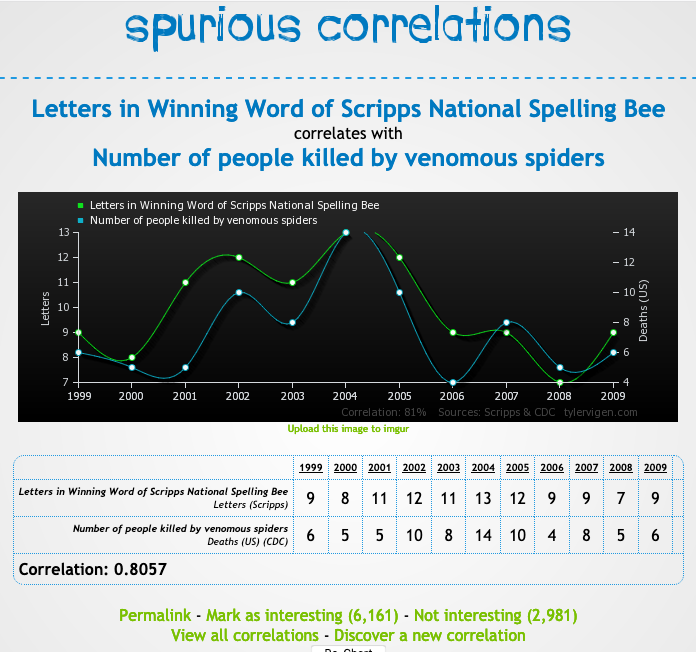
\includegraphics[width=.75\textheight]{graphics/spiders_spelling}
        }
    };
  
\end{tikzpicture}

\cite{spurious-spiders-spelling}
\end{frame}

\begin{frame}
\frametitle{Why causation matters}
\centering
\begin{tikzpicture}

    \node[inner sep=0pt] (med_caption) at (0,0) {
            Because A / B testing is hard.
    };
    \node[inner sep=0pt, below=0.5cm of med_caption] (med)  {
        \fbox{
            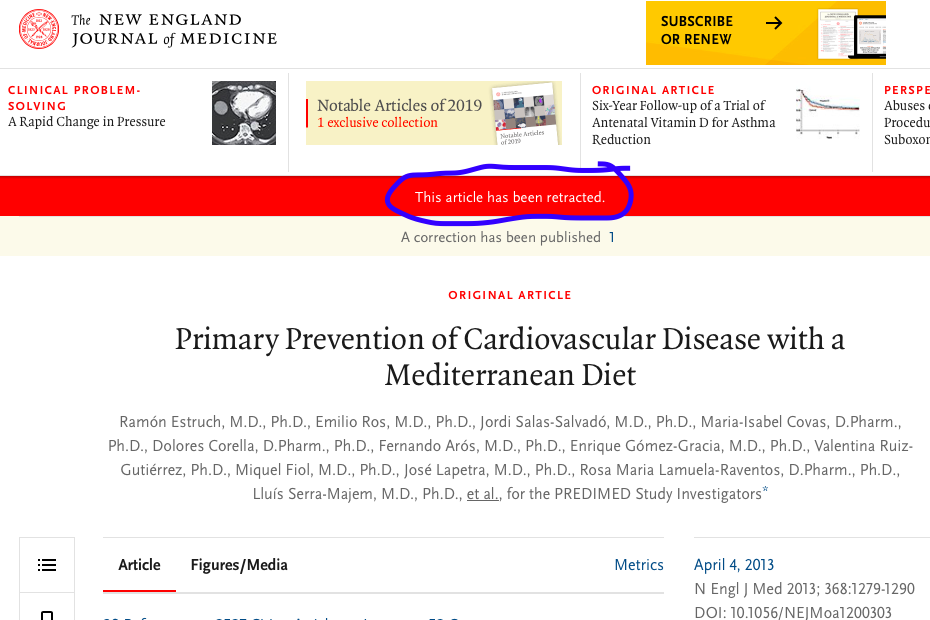
\includegraphics[width=.9\textheight]{graphics/mediterranean}
        }
    };
     
\end{tikzpicture}

\cite{estruch2013primary}
\end{frame}

\begin{frame}
\frametitle{A brief, biased history of causality}
\begin{itemize}
\item Aristotle, 384 - 322 BC
\item Isaac Newton, 1643 - 1727 AD
\item David Hume, 1711 - 1776 AD
\item Francis Galton, 1822 - 1900 AD, Karl Pearson, 1857 - 1936 AD
\item Judea Pearl, b. 1936 AD
\end{itemize}
\end{frame}

\begin{frame}
    \frametitle{Counterfactuals and causality}

    The definitions in following slides are from \cite{pearl2007mathematics}.

\end{frame}

\begin{frame}
    \frametitle{The Structural Causal Model}
    A \emph{structural causal model} $M$ consists of two sets of variables $U, V$ and a set of functions $F$, where 
    
    \begin{itemize}
        \item $U$ are considered \emph{exogenous}, or background variables, 
        \item $V$ are the \emph{causal} variables, i.e. that can be manipulated, and
        \item $F$ are the functions that represent the process of assigning values to elements of $V$ based on other values in $U, V$, e.g. $v_i = f(u, v)$.
    \end{itemize}

    We denote by $G$ the graph induced on $U, V$ by the functions $F$, and call it the \emph{causal graph} of $(U, V, F)$.
\end{frame}

\begin{frame}
    \frametitle{The definition of ``do"}
\end{frame}
\begin{frame}
\frametitle{Judea Pearl's Rules of Causality}

Let $X$, $Y$ , $Z$ and $W$ be arbitrary disjoint sets of nodes in a DAG $G$. Let $G_\underline{X}$ be the graph obtained by removing all arrows pointing into (nodes of) $X$. 
Denote by $G_{\overline{X}}$ the graph obtained by removing all arrows pointing out of $X$. If, e.g. we remove arrows pointing out of $X$ and into $Z$, we the resulting graph is denoted by $G_{\underline{X} \overline{Z}}$

Rules
\begin{equation}
P(y | \jpdo(x), z, w) = P(y | \jpdo(x), w) \textrm{ if } (Y \ci Z | X, W)_{G_{\overline{X}}}
\end{equation}

\begin{equation}
P(y | \jpdo(x), \jpdo(z), w) = P(y | \jpdo(x), z, w) \textrm{ if } (Y \ci Z | X, W)_{G_{\overline{X} \underline{Z}}}
\end{equation}

\begin{equation}
P(y | \jpdo(x), \jpdo(z), w) = P(y | \jpdo(x), w) \textrm{ if } (Y \ci Z | X, W)_{G_{\overline{X} \overline{Z(W)}}},
\end{equation}

where $Z(W)$ is the et of $Z$-nodes that are not ancestors of any $W$-node in $G_\underline{X}$.


\end{frame}

\begin{frame}[allowframebreaks]
    \frametitle{References}
    \bibliographystyle{amsalpha}
    \bibliography{../../references.bib}
\end{frame}

\end{document}